\documentclass[a4paper,14pt]{extarticle}
\usepackage[utf8]{inputenc}
\usepackage[russian]{babel}
\usepackage{graphicx}
\usepackage[top=0.8in, bottom=0.8in, left=0.8in, right=0.8in]{geometry}
\usepackage{pgfplots}
\usepackage{amsmath}
\usepackage{setspace}
\usepackage{titlesec}
\usepackage{float}
\usepackage{chngcntr}
\usepackage{pgfplots}
\usepackage{amsfonts}
\usepackage{pgfplotstable}
\usepackage{multirow}
\usepackage{karnaugh-map}
\usepackage{tikz,xcolor}
\usepackage{listings}
\usepackage{txfonts}

\titleformat{\section}[hang]
  {\bfseries}
  {}
  {0em}
  {\hspace{-0.4pt}\large \thesection\hspace{0.6em}}
  
  
\titleformat{\subsection}[hang]
  {\bfseries}
  {}
  {0em}
  {\hspace{-0.4pt}\large \thesubsection\hspace{0.6em}}

\newcommand{\nx}{\overline{x}}
\newcommand{\p}{0.31}
\newcommand{\scale}{1.4}

\counterwithin{figure}{section}
\counterwithin{equation}{section}
\counterwithin{table}{section}

\lstdefinestyle{CStyle}{
    basicstyle=\footnotesize,
    breakatwhitespace=false,         
    breaklines=true,                 
    captionpos=b,                    
    keepspaces=true,                 
    numbers=left,                    
    numbersep=5pt,                  
    showspaces=false,                
    showstringspaces=false,
    showtabs=false,                  
    tabsize=2,
    language=C
}

\begin{document}
\begin{titlepage}
\centering
\small Балтийский государственный технический университет «Военмех» им. Д.Ф.Устинова \\
\vspace{3cm}
\normalsize Кафедра И5\\
«Информационные системы и программная инженерия»\\
\vspace{3cm}
\textbf{Практическое задание №2}\\
по дисциплине Основы программирования на тему\\ 
\textbf{«Ветвления и циклы»}\\
\begin{center}
{\large\bf Вариант 14}
\end{center}
\vfill

\begin{flushleft}
\textbf{Выполнил:}
\hfill {Мальцев А.С.} \\
\hfill {Группа И595} \\
\vspace{1cm}
\textbf{Преподаватель:}
\hfill {Лазарева Т.И.} \\
\end{flushleft}
\vspace{3cm}

{\centering Санкт-Петербург \\ 
\vspace{0.15cm}
2019}
\end{titlepage}

\section{Цель работы}
Познакомиться с функциями из математической библиотеки, освоить операции отношения и логические операции, научиться грамотно программировать базовые алгоритмические структуры «ветвление» и «цикл».

\section{Ход работы}
\subsection{Задание 1}
Вычислить значение функции\\
\begin{equation*}
f(m,n) = 
 \begin{cases}
   \displaystyle\frac 5 m - \frac n 5 \text{, если $ n > -5, m \neq 0$}\\
   3m + n^2 \text{, если $ n \leq -5$}\\
   2mn \text{ в остальных случаях}
 \end{cases}
\end{equation*}
используя тернарный оператор.\\
\textit{Исходные данные:} так как значения m и n могут быть любыми, объявим соответствующие переменные типа double.\\
\textit{Результирующие данные:} значение функции f также типа double.\\
\begin{center}
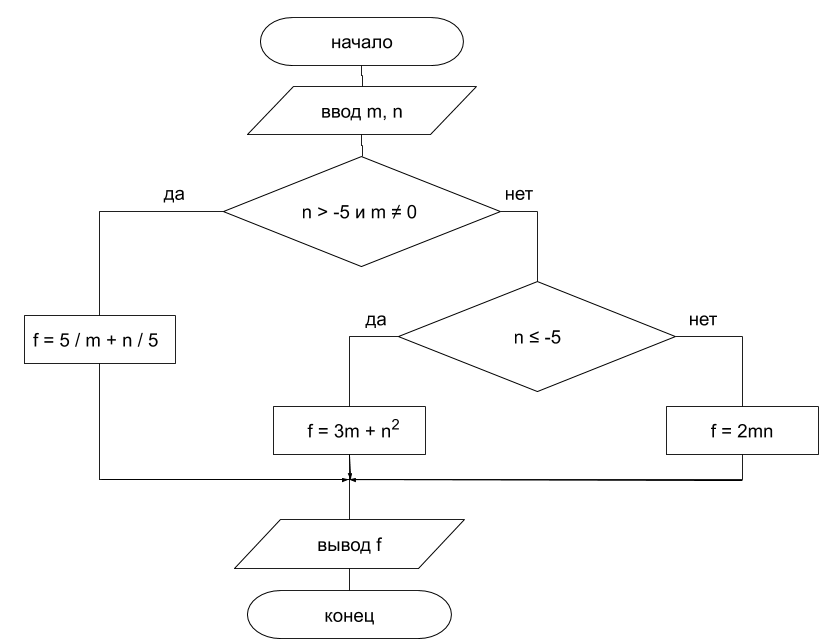
\includegraphics[scale=0.6]{lab2-1.png}
Схема программы
\end{center}
\lstinputlisting[language=c, frame=single, caption=Программа первого задания, label=lab2_2, style=CStyle]{../firstTask.c}
\begin{center}
\begin{tabular}{|c|c|}
\hline
Исходные данные & Вывод программы\\
\hline
m = 2, n = 4 & f = 1.700000\\
m = 3, n = -8 & f = 73.000000\\
m = 0, n = 0 & f = 0.000000\\
\hline
\end{tabular}\\
\end{center}

\subsection{Задание 2}
Вычислить значение функции
$S = \displaystyle\frac{ \sin \alphaup^3 + 2\cos^2\betaup }{\sqrt{2,5\alphaup + 3\betaup  + \sqrt{2}}\ln \betaup }$\\
\textit{Исходные данные:} типы $\alphaup$ и $\betaup$ не указаны в задании, поэтому будут double.\\
\textit{Результирующие данные:} значение функции S также типа double.
\vspace{0.5cm}
\begin{center}
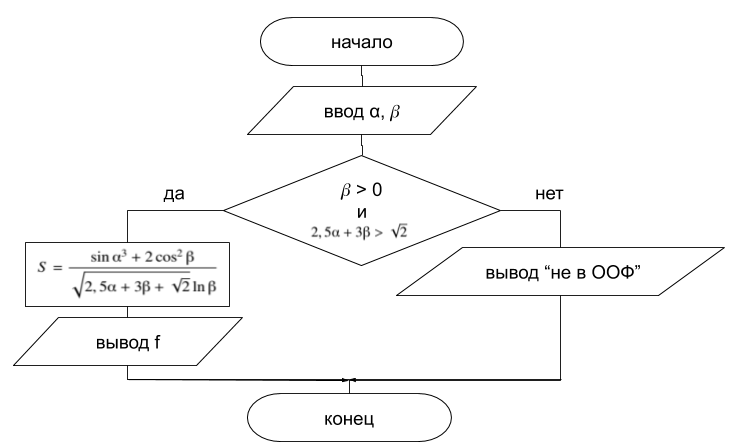
\includegraphics[scale=0.6]{lab2-2.png}
Схема программы
\end{center}
\lstinputlisting[language=c, frame=single, caption=Программа второго задания, label=lab2_2, style=CStyle]{../secondTask.c}

\subsection{Задание 3}
В финале шашечной партии остались белая дамка и две черные пешки, позиции которых известны. Ход белых. Сможет ли дамка «срубить» хотя бы одну пешку?
\begin{center}
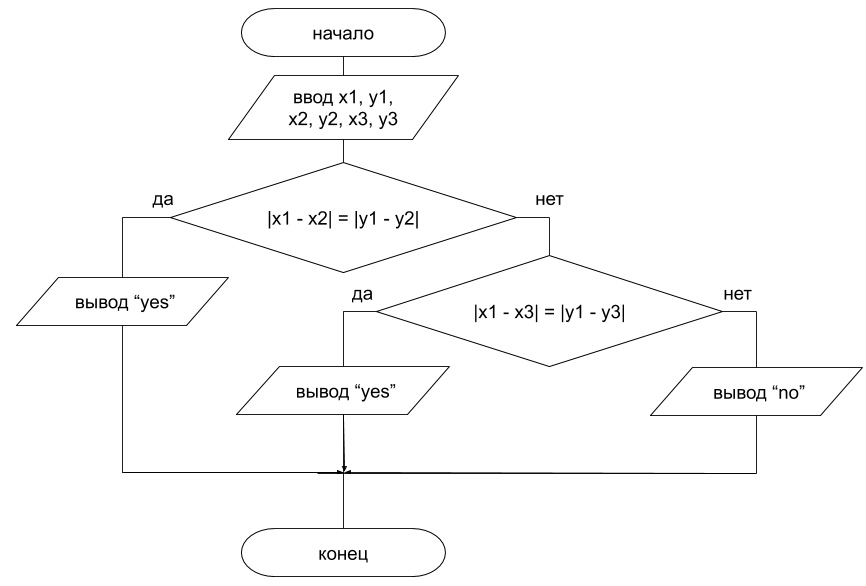
\includegraphics[scale=0.6]{lab2-3.png}\\
Схема программы
\end{center}
\lstinputlisting[language=c, frame=single, caption=Программа третьего задания, label=lab2_2, style=CStyle]{../thirdTask.c}

\subsection{Задание 4}
Составить программу для определения, в каких двузначных числах удвоенная сумма цифр равна их произведению.
\begin{center}
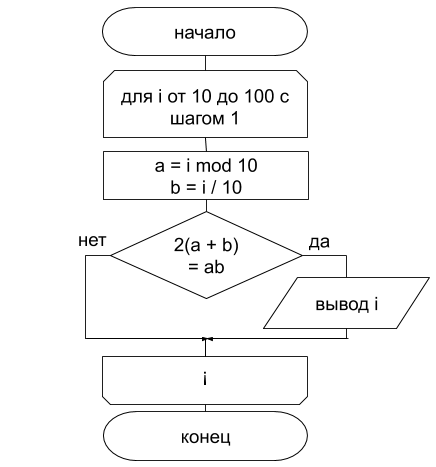
\includegraphics[scale=0.6]{lab2-4.png}\\
Схема программы
\end{center}
\lstinputlisting[language=c, frame=single, caption=Программа четвертого задания, label=lab2_2, style=CStyle]{../fourthTask.c}

\subsection{Задание 5}
Несколько деталей должны последовательно пройти обработку на каждом из трех станков. Продолжительности обработки каждой детали на каждом станке вводятся группами по три числа до исчерпания ввода (признак окончания ввода – задание некорректной тройки чисел). Сколько времени займет обработка всех деталей, если на каждом станке они могут обрабатываться только поштучно?
\begin{center}
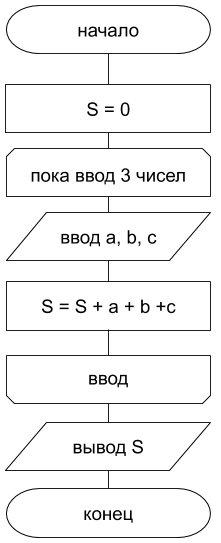
\includegraphics[scale=0.6]{lab2-5.png}\\
Схема программы
\end{center}
\lstinputlisting[language=c, frame=single, caption=Программа четвертого задания, label=lab2_2, style=CStyle]{../fivthTask.c}

\subsection{Задание 6}
Получить число, образованное записью цифр исходного числа N в обратном порядке.
\begin{center}
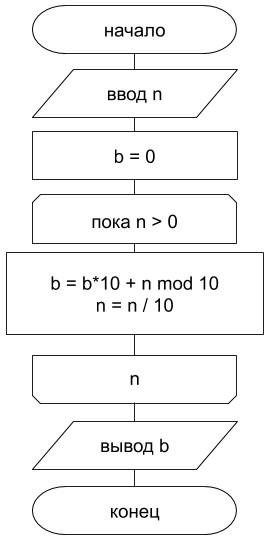
\includegraphics[scale=0.6]{lab2-6.png}\\
Схема программы
\end{center}
\lstinputlisting[language=c, frame=single, caption=Программа четвертого задания, label=lab2_2, style=CStyle]{../sixthTask.c}

\subsection{Задание 7}
Вычислить значение суммы членов бесконечного ряда\\
$S = ln x + 2[\frac {a} {2x+a} + \frac {a^3} {3(2x+a)^3} + \frac {a^5} {5(2x+a)^5}
+ ... + \frac {a^{2n-1}} {(2n-1)(2x+a)^{2n-1}} + ...]$
\begin{center}
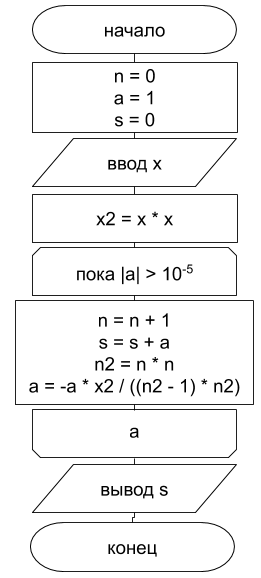
\includegraphics[scale=0.6]{lab2-7.png}\\
Схема программы
\end{center}
\lstinputlisting[language=c, frame=single, caption=Программа четвертого задания, label=lab2_2, style=CStyle]{../seventhTask.c}

\subsection{Задание 8}
В программе смоделирован арифметический цикл с помощью оператора цикла for.
\begin{center}
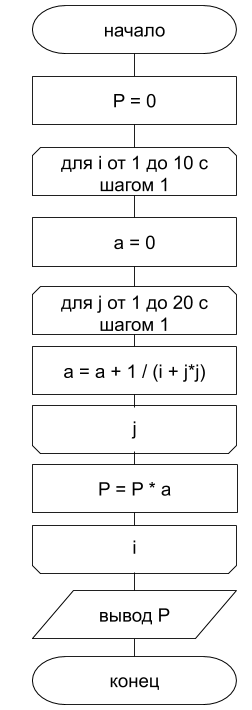
\includegraphics[scale=0.6]{lab2-9.png}\\
Схема программы
\end{center}
\lstinputlisting[language=c, frame=single, caption=Программа четвертого задания, label=lab2_2, style=CStyle]{../eightTask.c}

\subsection{Задание 9}
В программе смоделирован арифметический цикл с помощью оператора цикла for.
\begin{center}
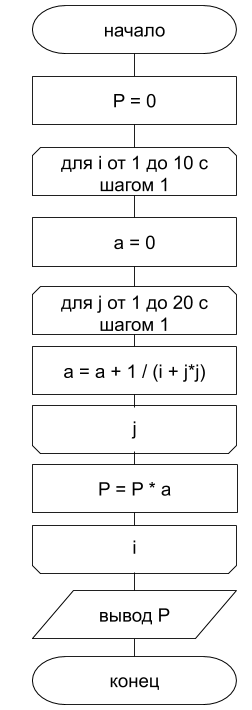
\includegraphics[scale=0.6]{lab2-9.png}\\
Схема программы
\end{center}
\lstinputlisting[language=c, frame=single, caption=Программа четвертого задания, label=lab2_2, style=CStyle]{../ninthTask.c}


\end{document}
